\documentclass[11pt]{amsart}
\usepackage{researchmacros}
\usepackage{ytableau}
\usepackage{mathtools}
\usepackage{enumitem}
\usepackage{tikz}
\usetikzlibrary{cd}
\usepackage[all]{xy}
\usepackage[vcentermath]{youngtab}

\usepackage{fullpage}


\usepackage{pifont}
\newcommand{\cmark}{\ding{51}}%
\newcommand{\xmark}{\ding{55}}%
\newcommand{\done}{\rlap{$\square$}{\raisebox{2pt}{\large\hspace{1pt}\cmark}}%
\hspace{-2.5pt}}



\newtheorem{theorem}{Theorem}[section] % 1st argument is your name for it
\newtheorem{lemma}[theorem]{Lemma}     % 2nd argument is what is printed
\newtheorem{corollary}[theorem]{Corollary}
\newtheorem{proposition}[theorem]{Proposition}
%To control the numbering sequence of these environments, see
%Lamport's book on LaTeX [2, p. 193].




\theoremstyle{definition}
\newtheorem{conjecture}[theorem]{Conjecture}  % 2nd argument is what is printed
\newtheorem{definition}[theorem]{Definition}
\newtheorem{remark}[theorem]{Remark}
\newtheorem{problem}[theorem]{Problem}
\newtheorem{question}[theorem]{Question}
\newtheorem{example}[theorem]{Example}





\title{A Hall--Littlewood expansion for \\$\Delta$--Springer varieties}
\author{Sean T. Griffin}

%\thanks{Sean T. Griffin was partially supported by NSF Grant DMS-1439786 while in residence at the Institute for Computational and Experimental Research in Mathematics in Providence, RI, during the Spring 2021 semester.}
\address{Department of Mathematics, University of California Davis, Davis, CA, USA}
\email{stgriffin@ucdavis.edu}




\date{\today}



\renewcommand{\top}{\mathrm{top}}
\newcommand{\std}{\mathrm{std}}
\newcommand{\conv}{\mathrm{conv}}
\newcommand{\sch}{\mathfrak{S}}
\newcommand{\init}{\mathrm{init}}
\newcommand{\Inv}{\mathrm{Inv}}
\newcommand{\st}{\,|\,}
\newcommand{\vspan}{\mathrm{span}}
\newcommand{\bA}{\mathbb{A}}
\newcommand{\Fl}{\mathrm{Fl}}
\newcommand{\GL}{\mathrm{GL}}
\newcommand{\Hilb}{\mathrm{Hilb}}
\newcommand{\Frob}{\mathrm{Frob}}
\newcommand{\la}{\lambda}
\newcommand{\im}{\mathrm{im}}
\newcommand{\SYT}{\mathrm{SYT}}
\newcommand{\sort}{\mathrm{sort}}
\newcommand{\fl}{\mathrm{f\hspace{0.25pt}l}}
\newcommand{\ufl}{\mathrm{ufl}}
\newcommand{\inv}{\mathrm{inv}}
\newcommand{\Hom}{\mathrm{Hom}}
\newcommand{\sh}{\mathrm{sh}}
\newcommand{\bx}{\mathbf{x}}
\newcommand{\fgl}{\mathfrak{gl}}
\newcommand{\ft}{\mathfrak{t}}
\newcommand{\rk}{\mathrm{rk}}
\newcommand{\Fq}{\mathbb{F}_q}
\newcommand{\bk}{\Bbbk}
\DeclareMathOperator{\IPRD}{IPRD}
\DeclareMathOperator{\Gr}{Gr}
\DeclareMathOperator{\coinv}{coinv}









%%%% commenting %%%%
\newcommand{\SG}[1]{{\color{red}#1}}




%\usepackage[inline]{showlabels}
\begin{document}
\maketitle


\begin{abstract}
    We give a positive Hall--Littlewood expansion formula for the graded Frobenius characteristic of the cohomology ring of a $\Delta$-Springer variety. We do this by interpreting the Frobenius characteristic in terms of counting points over a finite field $\mathbb{F}_q$ and decomposing the $\Delta$-Springer variety into dimensionally-shifted copies of Springer fibers.
\end{abstract}


%%%%%%%%%%%%%%%%%%%%%%%%%%%%
\section{Background}\label{sec:Background}
%%%%%%%%%%%%%%%%%%%%%%%%%%%%


\subsection{Flag varieties and Schubert cells}\label{subsec:Flags}

Given a complex vector space $V=\bC^K$, a \textbf{partial flag} is a nested sequence of vector subspaces of $V$,
\begin{align}
    V_\bullet = (V_1\subset V_2\subset\dots\subset V_m).
\end{align}
Given a composition $\alpha = (\alpha_1,\dots, \alpha_m)$ with $\alpha_i>0$ for all $i$ and $\alpha_1+\cdots+\alpha_m \leq \dim(V)$,  define the \textbf{partial flag variety} to be the set of partial flags of $V$ such that the dimensions of the successive quotients $V_i/V_{i-1}$ are recorded by the parts of $\alpha$, so
\begin{align}
    \Fl^{\alpha}(V) \coloneqq \{V_\bullet = (V_1\subset\dots\subset V_m) \st  V_i\subset V,\, \dim(V_i/V_{i-1}) = \alpha_i\text{ for }i\leq m\}.
\end{align}
In the case when $K=n$ and $\alpha = (1^n)$, we recover the \textbf{complete flag variety}, denoted by $\Fl(n) = \Fl^{(1^n)}(\bC^n)$.  The (partial) flag variety is realized as a projective algebraic variety as $G/P^{\alpha}$, where $G=GL_K(\bC)$ and $P^\alpha$ is a parabolic subgroup determined by $\alpha$.

From here on, we focus on the case where $\alpha=(1^n)$ for some $n\leq K$.  Let $f_1,f_2,\dots,f_K$ be the standard ordered basis of $\bC^K$.  Given an injective map $w:[n]\rightarrow[K]$, let the {\bf coordinate flag} $F_\bullet^{(w)}$ be defined by setting $F^{(w)}_p=\vspan\{f_{w(1)},\ldots, f_{w(p)}\}$ for all $p$, $1\leq p\leq n$.  Note that $G=GL_K(\mathbb{C})$ acts on $\Fl^\alpha(\bC^K)$ via its action on $\bC^K$ and so does its subgroup $B\subseteq G$ of upper-triangular matrices.
Now define the {\bf Schubert cell} $C_w$ to be the $B$ orbit of $F^{(w)}_\bullet$ and the {\bf Schubert variety} $X_w=\overline{C_w}$ to be its closure.  The Schubert cells form an affine paving (in fact a cell decomposition as a CW-complex) of the partial flag variety.

There are several other descriptions of the Schubert cells and Schubert varieties that will be helpful.  Given any $V_\bullet\in C_w$, for each $p$, $1\leq p\leq K$, there exists a unique vector $v_p\in V_p\setminus V_{p-1}$ such that
\begin{equation} \label{eq:SchubCellCoords}
v_p=f_{w(p)}+\sum_{h=1}^{w(p)-1} \alpha_{h,p} f_h,
\end{equation}
where $\alpha_{h,p}=0$ if $h\in\{w(1),\ldots,w(p-1)\}$.  Note $V_p=\vspan\{v_1,\ldots,v_p\}$.  The $\alpha_{h,p}$ that are not required to be 0 can be taken as algebraically independent coordinates on $C_w$, considered as a locally closed subvariety of $\Fl_{(1^n)}(\bC^K)$.

Schubert cells and Schubert varieties can also be described in terms of intersection conditions with respect to the {\bf base flag} $F_\bullet \coloneqq F_\bullet^{(\iota)}$, where $\iota : [K]\to[K]$ is the identity map. To be precise, $F_p=\vspan\{f_1,\ldots,f_p\}$ for all $p$, $1\leq p\leq n$.  Given an injective map $w : [n]\to [K]$, we have the \textbf{Schubert cell}
\begin{align} \label{eqn:SchubCellDef}
 C_w \coloneqq \{V_\bullet \in \Fl^{(1^n)}(\bC^K) \st \dim(V_i\cap F_p) = \#\{j\leq i \st w(j)\leq p\}\}
\end{align}
and the \textbf{Schubert variety}
\begin{align}
    X_w \coloneqq \{V_\bullet \in \Fl^{(1^n)}(\bC^K) \st \dim(V_i\cap F_p) \geq \#\{j\leq i\st w(j)\leq p\}\}.
\end{align}

Since the Schubert cells $C_w$ form an affine paving, the Schubert classes $\{[X_w] \st w:[n]\to [K] \text{ injective}\}$ form a basis of the cohomology ring $H^*(\Fl^{(1^n)}(\bC^K))$. (See Lemma \ref{lem:OddCohVanishes}.)



\subsection{Chern classes} 

Given a complex vector bundle $E$ on a paracompact Hausdorff space $X$, the $i$-th Chern class of $E$ is a distinguished cohomology class $c_i(E)\in H^{2i}(X)$, with $c_0(E) = 1$ by definition. The Chern classes are invariants of the vector bundle, in the sense that if two vector bundles on $X$ are isomorphic, then their Chern classes agree.  

The sum of the Chern classes of a vector bundle $c(E) \coloneqq 1+c_1(E) + c_2(E) +\cdots$ is called the {\bf total Chern class} of $E$. It has the following useful properties.
\begin{itemize}
    \item Naturality: For any continuous map $f : X \to Y$ and any complex vector bundle $E$ on $Y$, we have $f^*(c(E)) = c(f^*(E))$, where the first $f^*$ is the map on cohomology and $f^*(E)$ is the pullback of $E$.
    \item Additivity: Given a short exact sequence of vector bundles $0\to E'\to E\to E''\to 0$ on $X$, we have
    \begin{align}
        c(E) = c(E')c(E''),
    \end{align}
    where multiplication is via the cup product on cohomology.
    \item Vanishing: If $r$ is the rank of $E$ as a complex vector bundle, then $c_i(E) = 0$ for all $i>r$.
    \item Triviality: If $E \cong \bC^r \times X$, a trivial vector bundle, then $c(E) = 1$.
\end{itemize}

In the case where $X = \Fl(n)$, for each $j$, there is the tautological vector bundle $\widetilde V_j$ whose fiber over $V_\bullet = (V_1,\dots, V_n)$ is the vector space $V_{j}$. Borel~\cite{Borel} proved that the classes $-c_1(\widetilde V_j/\widetilde V_{j-1})$ generate the cohomology ring $H^*(\Fl(n))$ as a graded algebra. Moreover, there is an isomorphism of graded algebras
\begin{align}\label{eq:BorelTheorem}
    H^*(\Fl(n)) \cong \frac{\bZ[x_1,\dots, x_n]}{\langle e_1(x_1,\dots, x_n),\dots, e_n(x_1,\dots, x_n)\rangle}
\end{align}
identifying $-c_1(\widetilde V_j/\widetilde V_{j-1})$ with $x_j$, where each variable $x_j$ is considered to have degree $2$.
The quotient ring on the right-hand side of \eqref{eq:BorelTheorem} is also known as the \textbf{coinvariant ring}.





\subsection{Affine paving}

Given a complex algebraic variety $X$, an {\bf affine paving} of $X$ is a sequence of closed subvarieties
\begin{align} \label{eq:affine-paving}
    X_0 \subseteq X_1\subseteq \cdots \subseteq X_m = X
\end{align}
of $X$ such that $X_i\setminus X_{i-1} \cong \bigsqcup_j A_{i,j}$ for some locally closed subspaces $A_{i,j}$, where for all $i,j$, $A_{i,j}\cong \bC^k$ for some $k$. The affine spaces $A_{i,j}$ are called the {\bf cells} of the affine paving.

When $X$ is compact, an affine paving gives us a convenient basis of the cohomology groups of $X$. The following two lemmata are standard (see for example~\cite{Hotta-Springer}), whereas the third is less standard but will be very useful for us.

\begin{lemma}\label{lem:OddCohVanishes}
Suppose $X$ is a compact complex algebraic variety that has an affine paving. If $X_i\setminus X_{i-1} = \bigsqcup_{i,j} A_{i,j}$ is the decomposition of $X$ into affine spaces, then we have the following isomorphisms of groups
\begin{align}
    H_{2k}(X) &\cong \bZ \cdot \big\{[\overline{A_{i,j}}]\big\}_{i,j}, \\
    \label{eq:even-cohomology}
    H^{2k}(X) &\cong H_{2k}(X)^* \cong \bZ^{\#\{(i,j) \st \dim_\bC(A_{i,j}) = k\}}, \\ \label{eq:odd-cohomology}
    H^{2k+1}(X) & = 0,
\end{align}
for all $k\geq 0$, where $[\overline{A_{i,j}}]$ is the fundamental homology class of the cell closure. If ``compact'' is replaced by ``smooth'', then the vanishing \eqref{eq:odd-cohomology} holds for compactly-supported cohomology, so $H^{2k+1}_c(X) = 0$ for all $k\geq 0$.
\end{lemma}


\subsection{Springer fibers}

Given a partition $\lambda$ of $n$, let $N_\lambda$ be a $n\times n$ nilpotent matrix whose Jordan block sizes are recorded by $\lambda$. We say that $N_\lambda$ has {\bf Jordan type} $\lambda$. The {\bf Springer fiber} associated to $\lambda$ is
\begin{align}
    \cB^\lambda \coloneqq \{V_\bullet \in \Fl(n) \st N_\lambda V_i\subseteq V_{i-1} \text{ for all } i\leq n\}.
\end{align}
Springer constructed an action of $S_n$ on $H^*(\cB^\lambda)$ that does not come from an action on $\cB^\lambda$. We note that in this article, the action on the cohomology ring we consider differs from the one originally constructed by Springer by tensoring with the sign representation.

A remarkable property of this action is that it gives a geometric construction of all the finite dimensional irreducible representations of $S_n$. Indeed, the dimension of $\cB^\lambda$ as a complex variety is 
\begin{align}
    n(\lambda) \coloneqq \sum_i \binom{\lambda_i'}{2},
\end{align}
and the top nonzero cohomology group of $\cB^\lambda$ as an $S_n$-module is
\begin{align}
    H^{2n(\lambda)}(\cB^\lambda;\bQ) \cong S^\lambda,
\end{align}
where $S^\lambda$ is the irreducible representation of $S_n$ usually associated to $\lambda$.
Therefore, in Lie type A there is a bijection, known as the \textbf{Springer correspondence}, between Springer fibers and the irreducible $S_n$-modules up to isomorphism. 

Hotta and Springer~\cite{Hotta-Springer} proved that the map on cohomology induced by the inclusion $\cB^\lambda \subseteq \Fl(n)$,
\begin{align}
    H^*(\Fl(n)) \to H^*(\cB^\lambda),
\end{align}
is surjective and $S_n$-equivariant. Hence, by surjectivity the cohomology ring $H^*(\cB^\lambda)$ is generated by the cohomology classes $-c_1(\widetilde V_i/\widetilde V_{i-1})$. Here, we are abusing notation and writing $\widetilde V_i$ for the restriction of this vector bundle to $\cB^\lambda$. 

There is an explicit presentation of $H^*(\cB^\lambda)$ as a quotient ring extending Borel's theorem~\cite{dCP,Tanisaki}.  Let $\la'$ denote the conjugate partition to $\la$, and let $\la_i'$ be the parts of $\la'$, where $\la_i'\coloneqq 0$ for $i>\la_1$. Given $S\subseteq \{x_1,\dots, x_n\}$, define $e_d(S)$ to be the sum of all square-free products of variables in $S$ of degree $d$. Define the following ideal and quotient ring
\begin{align}
    I_\lambda &\coloneqq \langle e_d(S) \st S\subseteq \{x_1,\dots,x_n\},\, d > |S| - \la_n' - \cdots - \la_{n-|S|+1}' \rangle,\\
    R_\lambda &\coloneqq \bZ[x_1,\dots, x_n]/I_\lambda.
\end{align}
Here and throughout the paper, we consider $R_\lambda$ to be a graded ring where each variable $x_j$ has degree $2$. It follows from work of Tanisaki~\cite{Tanisaki} that there is an isomorphism of graded rings and graded $S_n$-modules
\begin{align}
    H^*(\cB^\lambda) \cong R_\lambda
\end{align}
given by identifying the cohomology class $-c_1(\widetilde V_j/\widetilde V_{j-1})$ with the variable $x_j$.

For example, when $\lambda = (2,1)$, the ideal $I_\lambda$ is generated by $e_d(S)$ where $3\geq d>0$ and $|S|=3$, or $2\geq d>1$ and $|S| = 2$, so 
\begin{align}
I_{(2,1)} &= \big\langle x_1+x_2+x_3,\, x_1x_2+x_1x_3+x_2x_3,\, x_1x_2x_3,\, x_1x_2,\, x_1x_3,\, x_2x_3\big\rangle,
\end{align}
and $H^*(\cB^{(2,1)})\cong R_{(2,1)} = \bZ[x_1,x_2,x_3]/I_{(2,1)}$.


\subsection{Symmetric functions}

The representation theory of the group $S_n$ is closely related to the theory of symmetric functions.
A {\bf symmetric function} is a formal power series in the infinite variable set $\bx = \{x_1,x_2,\dots \}$ that is invariant under any permutation of the variables.
Given $\la$ an integer partition of $n$, which we write as $\la\vdash n$,  we denote by $\ell(\la)$ be the number of (nonzero) parts of $\la$. For each $\la \vdash n$, let $e_\la(\bx)$ and $s_\la(\bx)$ denote the \textbf{elementary symmetric function} and \textbf{Schur symmetric function} indexed by $\lambda$.  As $\lambda$ ranges over all partitions of all $n$, these form bases of the ring of symmetric functions. 

The Frobenius characteristic map, which we define next, gives a connection between symmetric functions and representations of $S_n$. Given $\la\vdash n$, let $S^\la$ be the irreducible $S_n$-module indexed by $\la$, also known as a \textbf{Specht module}. Suppose a finite-dimensional $S_n$ representation $V$ (over $\bQ$) decomposes as a direct sum of Specht modules
\begin{align}
V\cong \bigoplus_{\la\vdash n}(S^\la)^{c_\la}
\end{align}
for some nonnegative integers $c_\la$. The \textbf{Frobenius characteristic} of $V$ is then defined as the symmetric function
\begin{align}
\Frob(V) = \sum_{\la\vdash n} c_\la s_\la(\bx).
\end{align}
Given a graded $S_n$-module $V = \bigoplus_{i \geq 0} V_i$ with finite-dimensional direct summands $V_i$, the \textbf{graded Frobenius characteristic} of $V$ is
\begin{align}
\Frob(V;q) = \sum_{i\geq 0} \Frob(V_i)q^i.
\end{align}
We refer the reader to~\cite{Sagan} for more details.


\subsection{Counting points in Springer fibers over finite fields}

There is an alternative description of the graded Frobenius characteristic of $H^*(\cB_\lambda;\bQ)$ in terms of counting points in projected Springer fibers (or Steinberg varieties) over finite fields.

\begin{theorem}[Needs citation]
We have
\[
\Frob(H^*(\cB_\lambda;\bQ);q) = \sum_\mu |\cB_\lambda^\mu(\Fq)|\,m_\mu(\bx).
\]
\end{theorem}

Say more about the map involving the Hall algebra.


\subsection{The rings \texorpdfstring{$R_{n,\lambda}$}{Rn,lambda} and \texorpdfstring{$R_{n,\lambda,s}$}{Rn,lambda,s}}

We recall the definitions and properties of the rings $R_{n,\la}$ and $R_{n,\la,s}$ introduced by the first author in \cite{GriffinOSP}. These rings simultaneously generalize the cohomology ring of a Springer fiber $H^*(\cB^\lambda)$ and the Haglund--Rhoades--Shimozono ring
\begin{align}
    R_{n,k} = \frac{\bZ[x_1,\dots, x_n]}{\langle x_1^k,\dots, x_n^k,e_n,e_{n-1},\dots, e_{n-k+1}\rangle}.
\end{align}

\begin{definition}\label{def:RnLaDef}
Fix nonnegative integers $k\leq n$, a partition $\la\vdash k$, and a positive integer $s\geq \ell(\la)$. 
 The ideals $I_{n,\la}$ and $I_{n,\la,s}$ are defined by
 \begin{align}
     I_{n,\la} &= \langle e_d(S) \st S\subseteq \{x_1,\dots, x_n\}, \, d > |S| - \la_n' - \cdots - \la_{n-|S|+1}'\rangle,\\
     I_{n,\la,s} &= I_{n,\la} +  \langle x_1^s,\dots, x_n^s\rangle.
 \end{align}
 The rings $R_{n,\la}$ and $R_{n,\la,s}$ are the corresponding quotients
 \begin{align}
 R_{n,\la} &= \bZ[x_1,\dots, x_n]/I_{n,\la},\\
 R_{n,\la,s} &= \bZ[x_1,\dots, x_n]/I_{n,\la,s}.
 \end{align}
 \end{definition}
 The rings $R_{n,\la}$ and $R_{n,\la,s}$ are evidently graded by degree and carry an action of $S_n$ by permuting the variables. In~\cite{GriffinOSP}, it is shown that $R_{n,\la}$ in general has infinitely many nonzero graded components, whereas $R_{n,\la,s}$ always has finite rank.

The following two specializations of $R_{n,\la,s}$ will be particularly important to us.
\begin{itemize}
    \item When $n=k$, $R_{n,\la,s}$ specializes to the cohomology ring of a Springer fiber. Precisely, $I_{n,\la,s} = I_{\lambda}$ for any $s\geq \ell(\la)$; thus $R_{n,\la,s} = R_\la$ in this case.
    \item When $\la = (1^k)$ and $s=k$, $R_{n,\la,s}$ specializes to the Haglund--Rhoades--Shimozono ring. Indeed, we have $I_{n,(1^k),k} = I_{n,k}$; thus $R_{n,(1^k),k} = R_{n,k}$.
\end{itemize}

\begin{example}
Let $n=4$, $\lambda = (2,1)$, and $s=2$. Then the ideal $I_{4,(2,1)}$ is generated by the polynomials 
$e_d(S)$ for $S\subseteq \{x_1,\dots, x_4\}$ such that
\begin{equation*}
\begin{aligned}
	d &= 2 \text{ and }|S| = 4,\\
	d &= 4\text{ and }|S| = 4,\\
\end{aligned}
\qquad
\begin{aligned}
	d &= 3\text{ and }|S| = 4,\\
	d &= 3\text{ and }|S| = 3.
\end{aligned}
\end{equation*}
We have
\begin{align*}
    I_{4,(2,1)} 
    &= \big\langle x_1x_2+x_1x_3+x_1x_4+x_2x_3+x_2x_4+x_3x_4,\\
    &\qquad x_1x_2x_3+x_1x_2x_4+x_1x_3x_4+x_2x_3x_4,\\ 
    &\qquad x_1x_2x_3x_4,\, x_1x_2x_3,\, x_1x_2x_4,\, x_1x_3x_4,\, x_2x_3x_4\big\rangle,
\end{align*}
and $I_{4,(2,1),2} = I_{4,(2,1)} + \langle x_1^2,x_2^2,x_3^2,x_4^2\rangle$. Finally, we have  $R_{4,(2,1)} = \bZ[x_1,x_2,x_3,x_4]/I_{4,(2,1)}$ and $R_{4,(2,1),2} = \bZ[x_1,x_2,x_3,x_4]/I_{4,(2,1),2}$.
\end{example}

Let $I_{n,\lambda,s}^\bQ$ be the ideal in $\bQ[x_1,\dots,x_n]$ given by the same generators as $I_{n,\lambda,s}$, and let $R_{n,\la,s}^\bQ = \bQ[x_1,\dots, x_n]/I_{n,\lambda,s}^\bQ$. 
There is a convenient basis of $R_{n,\la,s}^\bQ$ generalizing the \textbf{Artin basis} of the coinvariant ring, defined next. Set $\cA_{0,\emptyset,s} \coloneqq \{1\}$. Let the set $\cA_{n,\la,s}$ be defined recursively for $n\geq 1$ by
\begin{align}
    \cA_{n,\la,s} \coloneqq \bigsqcup_{i=1}^{\ell(\la)} x_n^{i-1} \cA_{n-1,\la^{(i)},s} \sqcup \bigsqcup_{i=\ell(\la)+1}^s x_n^{i-1} \cA_{n-1,\la,s},
\end{align}
where for $1\leq i \leq \ell(\la)$, $\la^{(i)}$ is the partition obtained by sorting the parts of \[(\la_1,\dots, \la_{i-1},\la_i-1,\la_{i+1},\dots, \la_{\ell(\la)})\]
and deleting a trailing zero if necessary.
It is shown in~\cite[Theorem 3.18]{GriffinOSP} that $\cA_{n,\la,s}$ is a $\bQ$-basis of $R_{n,\la,s}^\bQ$. In fact, it is straightforward to show that $\cA_{n,\la,s}$ is actually a $\mathbb{Z}$-basis of $R_{n,\la,s}$.





\begin{lemma}\label{lem:FreeZMod}
The ring $R_{n,\la,s}$ is a free $\bZ$-module, and the set $\cA_{n,\la,s}$ is a $\bZ$-basis of $R_{n,\la,s}$.
\end{lemma}
\begin{proof}
The proof of Lemma 3.14 in \cite{GriffinOSP} also proves that $\cA_{n,\la,s}$ is a $\bZ$-spanning set of $R_{n,\la,s}$. Since $\cA_{n,\la,s}$ is a $\bQ$-linearly independent subset of $R_{n,\la,s}^\bQ$, it is also a $\bZ$-linearly independent subset of $R_{n,\la,s}$, and $R_{n,\la,s}$ is free as a $\bZ$-module.
\end{proof}

Given $V = \bigoplus_{i\geq 0} V_i$ a graded free $\bZ$-module with graded pieces $V_i$ of finite rank $\mathrm{rk}(V_i)$, let the \textbf{Hilbert--Poincar\'e series} of the module $V$ be 
\begin{align}
    \Hilb(V;q) \coloneqq \sum_{i\geq 0} \mathrm{rk}(V_i)q^i.
\end{align}
Under our convention that $x_i$ has degree $2$ for all $i$, we have the following recursive formula for the Hilbert series, which follows immediately by Lemma~\ref{lem:FreeZMod}.
\begin{lemma}\label{lem:RHilbRecursion}
We have
\begin{align}
    \Hilb(R_{n,\la,s};q) = \sum_{i=1}^{\ell(\la)} q^{2(i-1)} \Hilb(R_{n-1,\la^{(i)},s};q) + \sum_{i=\ell(\la)+1}^s q^{2(i-1)} \Hilb(R_{n-1,\la,s};q).
\end{align}
\end{lemma}

Since the set of generators of the homogeneous ideal $I_{n,\la,s}$ is closed under the action of $S_n$ permuting the variables, $R_{n,\la,s}$ inherits the structure of a graded $S_n$-module. In order to prove our generalization of the Springer correspondence, we make use of a formula for the graded Frobenius characteristic of $R_{n,\la,s}^\bQ$ proven in~\cite{GriffinOSP}. We state the formula and define the associated combinatorial objects in Section~\ref{sec:IrreducibleComponents} where we need it.




%%%%%%%%%%%%%%%%%%%%%%%%%%%%
\section{An affine paving of the \texorpdfstring{$\Delta$}{Delta}-Springer variety}\label{sec:AffinePaving}
%%%%%%%%%%%%%%%%%%%%%%%%%%%%

In this section, we define a family of varieties $Y_{n,\lambda,s}$ that generalize the Springer fibers, which we call $\Delta$-Springer varieties. We construct an affine paving of $Y_{n,\lambda,s}$ by intersecting it with Schubert cells.
We show that this affine paving has an inductive structure that allows us to show $H^*(Y_{n,\lambda,s})$ and $R_{n,\lambda,s}$ have the same Hilbert--Poincar\'e series.

Our approach most closely resembles that of Tymoczko~\cite{Tymoczko-LinearConditions} for type A regular Hessenberg varieties, which was extended to arbitrary type by Precup~\cite{Precup-AffinePavings}. Our work is also inspired by  Spaltenstein~\cite[Chapitre II, Proposition 5.9]{Spaltenstein-book}, who gave an affine paving for the case of Springer fibers.  Similar constructions of affine pavings have also been given by Shimomura~\cite{Shimomura} and Fresse~\cite{Fresse}.  

Let $0\leq k\leq n$ be integers, let $\la\vdash k$, and let $s$ be a positive integer such that $\ell(\lambda) \leq s$. Define $\Lambda \coloneqq \Lambda(n,\lambda,s) \coloneqq (n-k+\lambda_1,\ldots,n-k+\lambda_s)$ a partition (where $\la_i=0$ for all $i>\ell(\la)$) of $K\coloneqq |\Lambda|=s(n-k)+k$. We define the $\Delta$-Springer variety, which is our main object of study.
\begin{definition}
Let $N_\Lambda$ be a nilpotent matrix of Jordan type $\Lambda$. Define the \textbf{$\Delta$-Springer variety}
\begin{align}
    Y_{n,\la,s}\coloneqq \{V_\bullet \in \Fl_{(1^n)}(\bC^K)\st N_\Lambda V_i\subseteq V_{i-1}\text{ for }i\leq n,\text{ and }N_\Lambda^{n-k}\bC^K\subseteq V_n\},
\end{align}
where $V_0\coloneqq 0$.
\end{definition}



\begin{remark}
Since $N_\Lambda$ is nilpotent, it can be checked that the set of partial flags $V_\bullet\in \Fl_{(1^n)}(\bC^K)$ satisfying the conditions $N_\Lambda V_i\subseteq V_{i-1}$ for $i\leq n$ is the same as the set of flags satisfying the conditions $N_\Lambda V_i\subseteq V_{i}$ for $i\leq n$. Therefore, the variety $Y_{n,\la,s}$ can alternatively be defined as the reduced scheme of points satisfying
\begin{align}
    Y_{n,\la,s} = \{V_\bullet \in \Fl_{(1^n)}(\bC^K) \st N_\Lambda V_i\subseteq V_{i} \text{ for }i\leq n,\text{ and }N_\Lambda^{n-k}\bC^K\subseteq V_n\}.
\end{align}
\end{remark}

\begin{remark}[Base case $n=0$]\label{rmk:BaseCase}
For clarity in induction proofs below, we describe the case $n=0$. In this case, we must have $k=0$, $\lambda = \emptyset$, and $s>0$ arbitrary. Therefore, the ideal $I_{0,\emptyset,s}$ has no generators, so $I_{0,\emptyset,s}=\langle 0\rangle$, and since $n=0$, the ring $R_{0,\emptyset,s}$ is the quotient of the $\bZ$-algebra with no generators, namely $R_{0,\emptyset,s} = \bZ/\langle 0\rangle = \bZ$. For the $\Delta$-Springer variety, we have that $\Fl(0)$ is a single point, which represents the trivial flag, and the $\Delta$-Springer variety is also a single point. Thus, $H^*(Y_{0,\emptyset,s}) = \bZ = R_{0,\emptyset,s}$.
\end{remark}


\begin{lemma}
\label{lem:ConjInd}
  The structure of $Y_{n,\la,s}$ as an algebraic variety is independent of the choice of $N_\Lambda$.
\end{lemma}

\begin{proof}
Let $N_\Lambda$ and $N_\Lambda'$ be two nilpotent matrices of Jordan type $\Lambda$, and let $Y_{n,\la, s}$ and $Y_{n, \la,s}'$ be the corresponding $\Delta$-Springer varieties. Since $N_\Lambda$ and $N_{\Lambda}'$ have the same Jordan type, there exists $g\in \GL_K(\bC)$ such that $N_\Lambda' = gN_\Lambda g^{-1}$. It follows that $g Y_{n,\lambda, s} = Y_{n,\lambda, s}'$ under the action of $\GL_K(\bC)$ on $\Fl_{(1^n)}(\bC^K)$.  In particular, $Y_{n, \la, s} \cong Y_{n, \la, s}'$.
\end{proof}







We denote by $[\Lambda]$ the Young diagram of $\Lambda$, following the English convention, considered as the set
\begin{equation}
[\Lambda]=\{(i,j)\mid 1\leq i\leq \ell(\Lambda), 1\leq j\leq \Lambda_i\},
\end{equation}
where $(i,j)$ is the cell in the $i$-th row from the top and the $j$-th column from the left.
The cells in column $n-k+1$ and to the right form a copy of the Young diagram of $\lambda$, which we denote by $[\lambda]$. 
We say that a cell $(i,j)$ of $[\Lambda]$ is on the \textbf{right edge} if $j=\Lambda_i$.
See Figure~\ref{fig:Lambda} for an illustration of $[\Lambda]$ and $[\lambda]$, where the cells in the right edge of $[\Lambda]$ are shaded. 


\begin{figure}
    \centering
    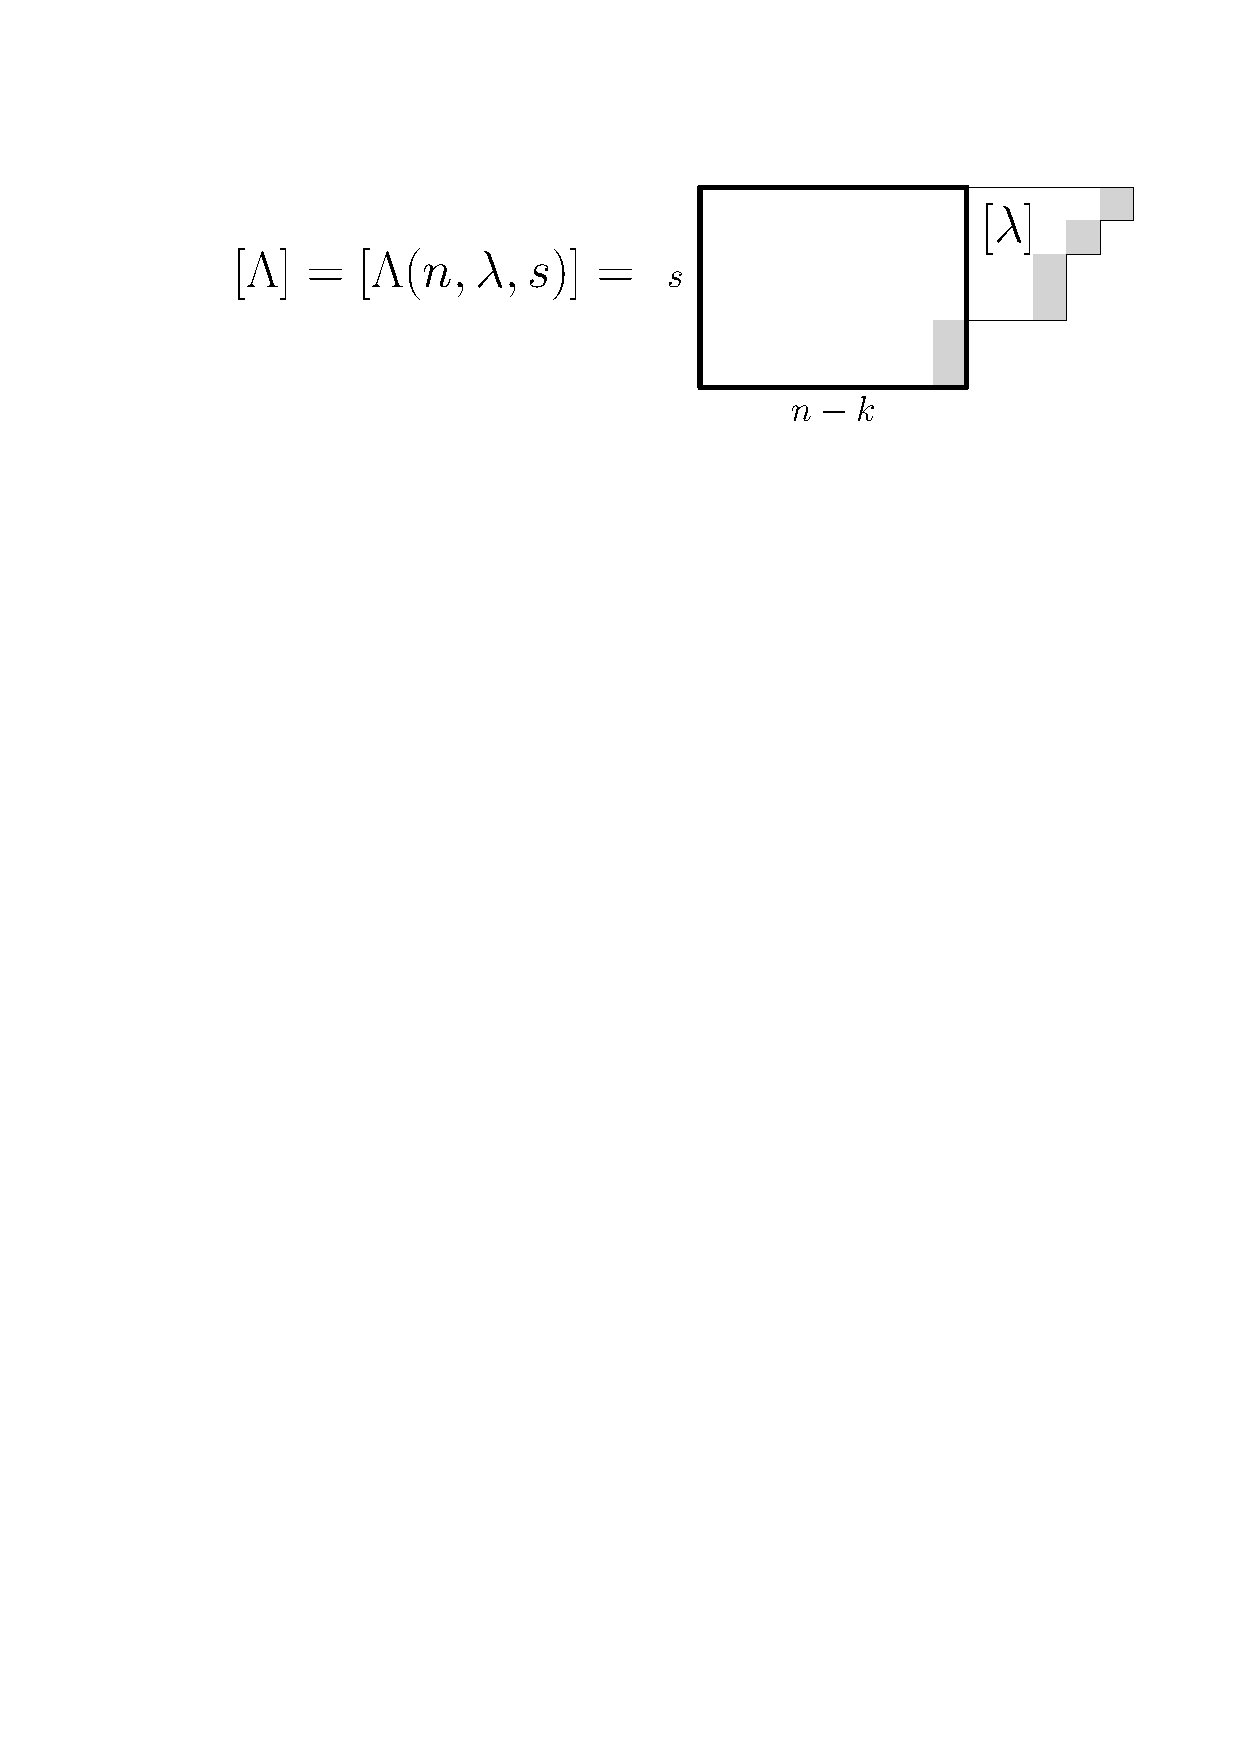
\includegraphics[scale=0.45]{Figures/LambdaExMain.pdf}
    \caption{The Young diagram $[\Lambda]$, which has a copy of $[\lambda]$ in the upper right corner, highlighted in bold. The cells in the right edge of $[\Lambda]$ are shaded.
    }
    \label{fig:Lambda}
\end{figure}


It will be convenient to specify particular choices for $N_\Lambda$, which we do next. For any filling $T:[\Lambda]\rightarrow \mathbb{Z}_{>0}$ of $[\Lambda]$ satisfying the following conditions,
\begin{enumerate}
\item[(S1)] $T$ is a bijection between $[\Lambda]$ and $\{1,2,\dots, K\}$,
\item[(S2)] $T$ restricts to a bijection between $[\lambda]$ and $\{1, 2, \ldots, k\}$,
\end{enumerate}
we define a variety $Y_{T}$, as follows.
Let $f_1,\ldots,f_K\in \mathbb{C}^K$ be the standard ordered basis, and let $F_p=\vspan\{f_1,\ldots,f_p\}$ for all $p$ with $1\leq p\leq K$. Define $N_T$ to be the nilpotent endomorphism such that for $(i,j)\in [\Lambda]$,
\begin{align}
N_T(f_{T(i,j)}) = 
\begin{cases} 
0 & \text{ if }(i,j)\text{ is on the right edge of }[\Lambda],\\
f_{T(i,j+1)} & \text{ otherwise.}
\end{cases}
\end{align}
Note that $N_T$ has Jordan type
$\Lambda$ by construction.  
Define
\begin{align}
    Y_T \coloneqq Y_{n,\lambda,s,T}\coloneqq \{V_\bullet\in\Fl_{(1^n)}(\mathbb{C}^K) \mid N_TV_i\subseteq V_{i-1}\text{ for all } i\text{, and } F_k\subseteq V_n\},
\end{align}
which is a specific instance of the variety $Y_{n,\la,s}$.

In order to ensure that the intersection of $Y_{T}$ with the Schubert decomposition of $\Fl_{(1^n)}(\bC^K)$ is a paving by affines,
we must first put further conditions on $T$. 
We say that $T$ is {\bf $(n,\lambda,s)$-Schubert compatible} if (S1), (S2), and the following conditions hold:
\begin{enumerate}
\item[(S3)] $T$ is decreasing along each row from left to right.
\item[(S4)] For all $(i,j)\in [\lambda]$, the label $T(i,j)$ is greater than all labels in column $j+1$.
\item[(S5)] The labels of $T$ in the right edge of $[\Lambda]$ form an increasing sequence when read from top to bottom.
\item[(S6)] Whenever $T(a,b)>T(c,d)$ for $b,d>1$, then $T(a,b-1)>T(c,d-1)$.
\end{enumerate}
If $n$, $\lambda$, and $s$ are obvious from context, we will simply say $T$ is {\bf Schubert compatible}.



\begin{figure}
    \centering
    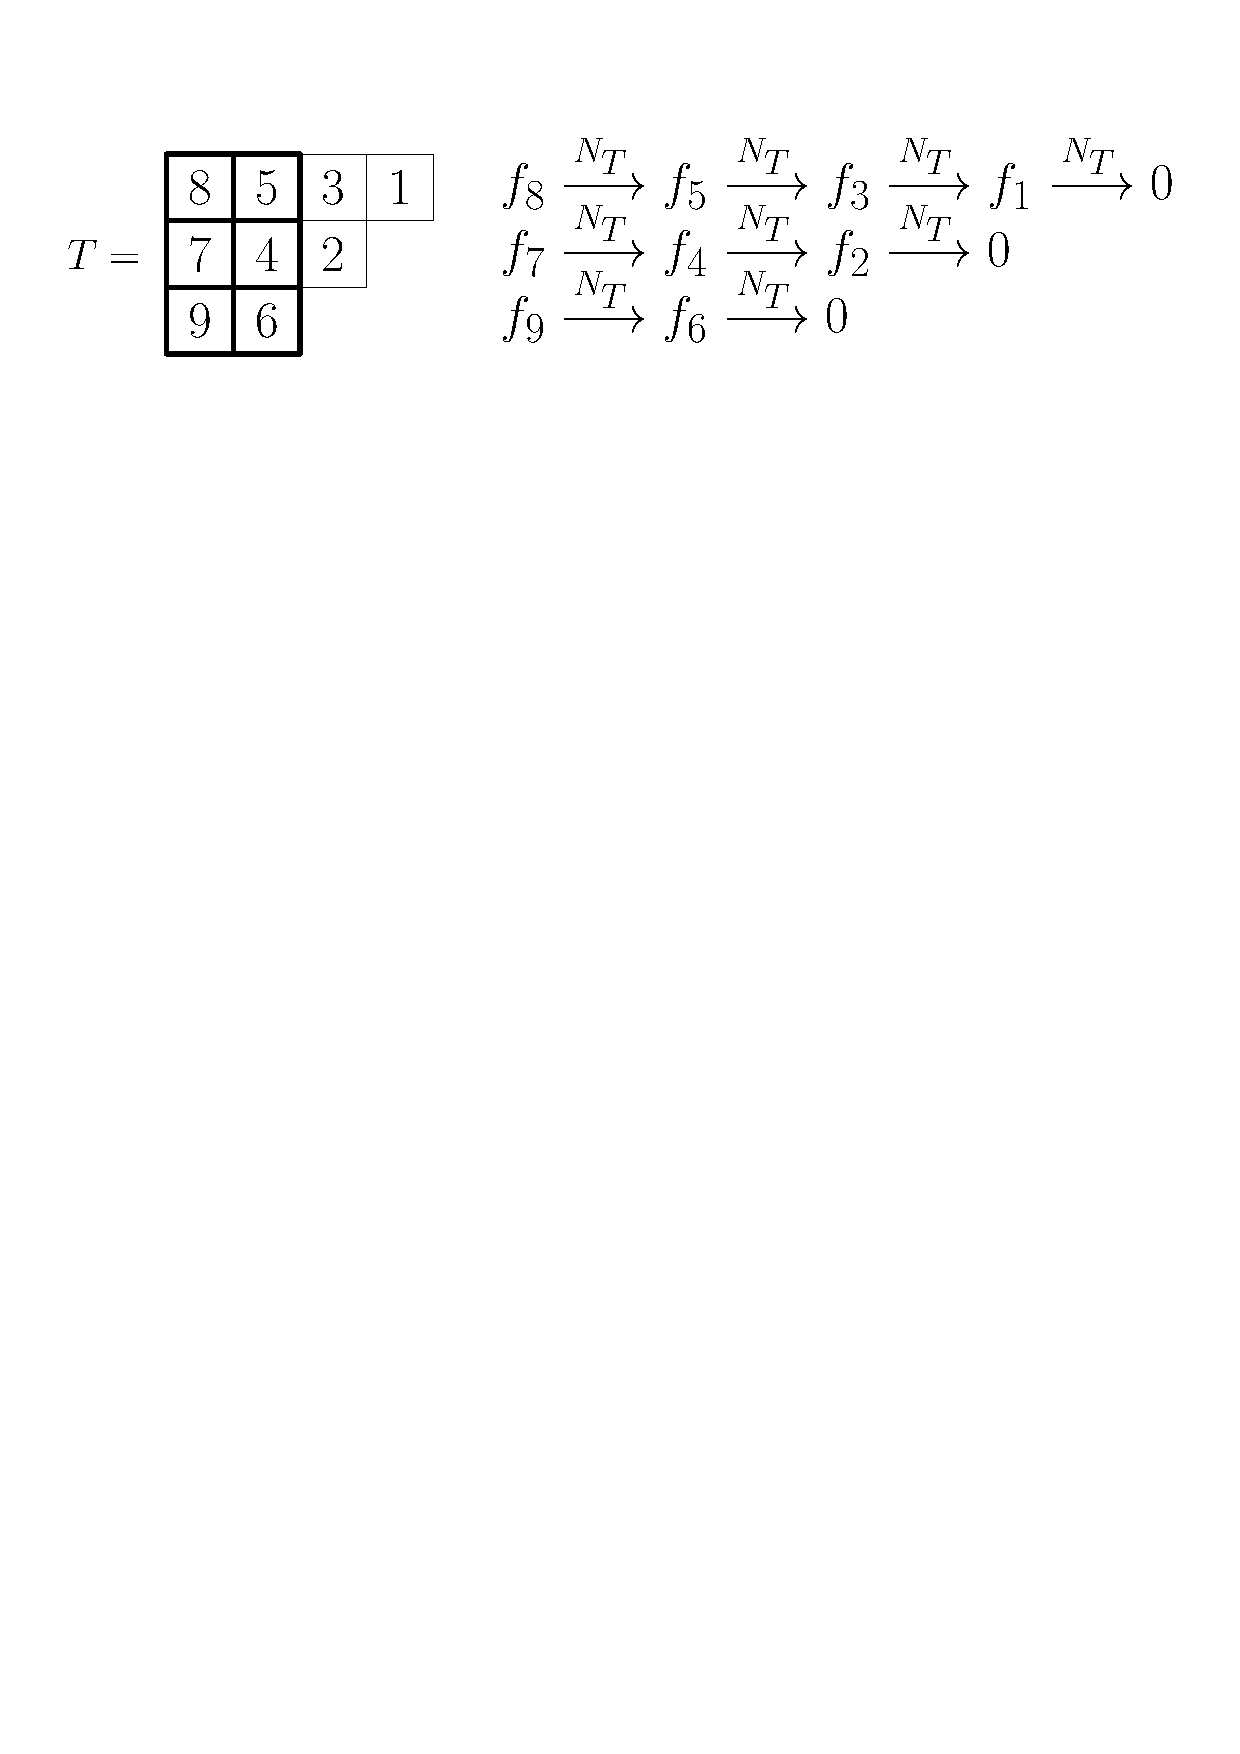
\includegraphics[scale=0.45]{Figures/SchubertCompatible.pdf}
    \caption{A Schubert-compatible filling $T$ of $\Lambda(5,(2,1),3)$ and the action of $N_T$ on the basis vectors.}
    \label{fig:SchubertCompatible}
\end{figure}

\begin{example}
Let $n=5$, $\lambda = (2,1)$, and $s=3$. Let $T$ be the Schubert-compatible filling of $\Lambda(5,(2,1),3)$ in Figure~\ref{fig:SchubertCompatible}. Then $Y_{5,(2,1),3,T}$ is the variety of partial flags $V_\bullet = (V_1,V_2,V_3,V_4,V_5)\in \Fl_{(1,1,1,1,1)}(\bC^9)$ such that the following conditions hold:
\begin{align}
N_T V_i &\subseteq V_{i-1} \text{ for } i \leq 5, \\
V_5 &\supseteq F_3 = \vspan\{f_1,f_2,f_3\}.
\end{align}
For example, the partial flag 
\begin{equation*}\label{eq:PartialFlag}
\vspan\{ f_1 \} \subset \vspan\{ f_1,f_2 \} \subset 
\vspan\{ f_{1},f_{2},f_{4} \} \subset \vspan\{ f_{1},f_{2},f_{3},f_{4} \} \subset \vspan\{ f_{1},f_{2},f_{3},f_{4},f_{7}\}.
\end{equation*}
is in $Y_{5,(2,1),3}$.
\end{example}


\begin{example}\label{ex:ReadingOrder}
We construct a Schubert-compatible filling $T$ for any shape $\Lambda$ as follows. 
Let the \textbf{reading order} of $[\Lambda]$ be the ordering of the cells given by scanning down the columns of $[\Lambda]$ from right to left. For $(i,j)\in [\Lambda]$, if $(i,j)$ is the $p$-th cell in the reading order, then let $T(i,j)=p$. We refer to $T$ as the filling of $[\Lambda]$ according to reading order. It can be checked that $T$ is a Schubert-compatible filling. See the left-most filling in Figure~\ref{fig:ReadingOrder} for an example of such a filling with $n=7$, $\lambda = (2,2)$, and $s=4$.
\end{example}

\begin{lemma}\label{lem:S6}
Suppose $T$ is a Schubert-compatible filling of $[\Lambda]$. If $(i,j)$ is not on the right edge of $[\Lambda]$, then 
\begin{equation}
N_T (F_{T(i,j)}\setminus F_{T(i,j)-1}) \subseteq F_{T(i,j+1)}\setminus F_{T(i,j+1)-1}.
\end{equation}
\end{lemma}

\begin{proof}
We have $N_T \, f_{T(i,j)} = f_{T(i,j+1)}$ by definition. Let $a$ and $b$ be indices such that $f_{T(a,b)}\in F_{T(i,j)}$, which means $T(a,b) < T(i,j)$. If $(a,b)$ is not on the right edge of $[\Lambda]$, by (S6) we have $T(a,b+1) < T(i,j+1)$, and hence $N_T\, f_{T(a,b)} = f_{T(a,b+1)}\in F_{T(i,j+1)}$. Otherwise, if $(a,b)$ is on the right edge, then $N_T\, f_{T(a,b)} = 0$. In either case, we have $N_T F_{T(i,j)} \subseteq F_{T(i,j+1)}$. 

If $v\in F_{T(i,j)}\setminus F_{T(i,j)-1}$, then the expansion of $v$ in the $f$ basis has a nonzero $f_{T(i,j)}$ coefficient. Therefore, the expansion of $N_T\, v$ in the $f$ basis has a nonzero $f_{T(i,j+1)}$ coefficient, so $N_T\, v\notin F_{T(i,j+1)-1}$. The lemma then follows.
\end{proof}



For $1\leq i \leq s$, define a {\bf flattening function} $\fl_T^{(i)}$ 
and a filling $T^{(i)}$ as follows.
If $i\leq \ell(\lambda)$, then $\fl_T^{(i)}$ is the unique order-preserving function with the following domain and codomain,
\begin{align}
    \fl_T^{(i)} : [K]\setminus\{ T(i,\Lambda_i) \} \to [K-1].
\end{align}
If $i> \ell(\lambda)$, then $\fl_T^{(i)}$ is the unique order preserving function
\begin{align}
    \fl_T^{(i)}: [K]\setminus(\{T(i,\Lambda_i)\}\cup \{T(i',1)\mid i'\neq i\}) \to [K-s].
\end{align}
Now if $i\leq \ell(\lambda)$, let $T^{(i)}$ be the filling obtained by deleting the last cell in row $i$, applying $\fl_T^{(i)}$ to the label in each cell, and reordering the rows so that the labels of the cells in the new right edge are increasing from top to bottom.
If $i>\ell(\lambda)$, we form $T^{(i)}$ in the same way except we also delete the cell $(i',1)$ and shift row $i'$ to the left by one unit for every $i'\neq i$ before applying $\fl_T^{(i)}$ to every label and reordering the rows.

\begin{example}
In Figure~\ref{fig:ReadingOrder} we have an example of a Schubert-compatible filling $T$ and the fillings $T^{(1)}$ and $T^{(3)}$. When constructing $T^{(3)}$, the cells labeled by $7,13,14$, and $16$ are deleted, and rows $1,2$ and $4$ are shifted left by one unit. The cells are relabeled as follows: $\fl_T^{(3)}(8)=7$, $\fl_T^{(3)}(9) = 8$, $\fl_T^{(3)}(10) = 9$, $\fl_T^{(3)}(11)=10$, $\fl_T^{(3)}(12) = 11$, and $\fl_T^{(3)}(15)=12$. Then rows $3$ and $4$ are swapped to obtain $T^{(3)}$. It can be checked that both $T^{(1)}$ and $T^{(3)}$ are Schubert compatible.
\end{example}

Recall that, given a partition $\lambda$, then $\lambda^{(i)}$ is defined to be the partition whose Young diagram is obtained from $[\lambda]$ by removing one box from the $i$-th row and then reordering the rows in decreasing order (by number of boxes) if necessary.

\begin{lemma}
The filling $T^{(i)}$ is of partition shape.  If $i \leq \ell(\lambda)$, then $T^{(i)}$ is $(n-1,\lambda^{(i)},s)$-Schubert compatible. If $i > \ell(\lambda)$, then $T^{(i)}$ is $(n-1,\lambda,s)$-Schubert compatible.
\end{lemma}

\begin{proof}
If $i\leq\ell(\la)$, the condition (S4) forces $T^{(i)}$ to have partition shape after sorting the rows by the labels in the right edge, and $T^{(i)}$ is of shape $\Lambda(n-1,\la^{(i)},s)$ since one box is removed from the $i$-th row of $\lambda$ and the rows are reordered in decreasing order.  If $i> \ell(\la)$, then $T^{(i)}$ is of shape $\Lambda(n-1,\la,s)$ since one box is removed from each row and, by (S2), any reordering only affects rows below the $\ell(\la)$-th row.  It also follows by construction that (S1) and (S2) hold for $T^{(i)}$.

The operations of deleting a cell, applying the flattening function to the labels, and possibly shifting a row to the left all preserve (S3), so $T^{(i)}$ has property (S3). Since (S4) only concerns labels of $[\lambda]$, and either all cells of $[\lambda]$ remain in place (except the one that is removed) or all cells of $[\la]$ are shifted left one column during the process of constructing $T^{(i)}$, we see $T^{(i)}$ also satisfies (S4). The property (S5) is automatically satisfied since we resort the rows by the label in the rightmost cell. Finally, $T^{(i)}$ satisfies (S6) since deleting a cell, relabeling, swapping rows, and shifting a row to the left all preserve the property (S6). Therefore, $T^{(i)}$ is Schubert compatible. 
\end{proof}




\begin{figure} 
    \centering
    \includegraphics[scale=0.45]{Figures/ReadingOrder.pdf}
    \caption{The Schubert-compatible filling $T$ of $[\Lambda] = [\Lambda(7,(2,2),4)]$ determined by reading order and the fillings $T^{(1)}$ and $T^{(3)}$, which are also Schubert compatible.}
    \label{fig:ReadingOrder}
\end{figure}





Recall that the set of injective maps $w:[n]\rightarrow [K]$ indexes the Schubert cells of $\Fl_{(1^n)}(\mathbb{C}^K)$.
\begin{definition}
Given $w:[n]\rightarrow[K]$ injective, we say that $w$ is {\bf admissible} with respect to $T$ if both of the following hold.
\begin{itemize}
    \item[(A1)] The image of the map $w$ contains $[k]$.
    \item[(A2)] For $i\leq n$, if $w(i)=T(a,b)$ for $(a,b)$ not on the right edge of $[\Lambda]$, then $T(a,b+1)\in \{w(1),\dots, w(i-1)\}$. 
\end{itemize}
\end{definition}

\begin{lemma}\label{lem:NonemptyIntersections}
Assume $T$ is a Schubert-compatible filling.  Then  $C_w\cap Y_{T}\neq\emptyset$ if and only if $w$ is admissible.
\end{lemma}



\begin{proof}
If $w$ is admissible, then the partial permutation flag $F^{(w)}_\bullet$ is in $C_w\cap Y_{T}$, so $C_w\cap Y_{T} \neq \emptyset$. Therefore, it suffices to prove that if $C_w\cap Y_{T}\neq\emptyset$, then $w$ is admissible.

Given an injective map $w: [n]\to [K]$, recall that 
\begin{align} \label{eqn:RecallSchubCellDef}
    C_w = \{V_\bullet \in \Fl_{(1^n)}(\bC^K) \st \dim(V_i\cap F_j) = \#\{p\leq i \st w(p)\leq j\}\}.
\end{align}
Given $V_\bullet\in \Fl_{(1^n)}(\bC^K)$, then $F_k\subseteq V_n$ if and only if $\dim(V_n\cap F_k) = k$. Therefore, $F_k\subseteq V_n$ for some $V_\bullet\in C_w$ if and only if (A1) holds.

Suppose $C_w\cap Y_{T}\neq\emptyset$, and let $V_\bullet \in C_w\cap Y_{T}$. Suppose there exists $i\leq n$ such that $w(i) = T(a,b)$ for some cell $(a,b)$ not on the right edge of $[\Lambda]$.
Then $\dim(V_i\cap F_{T(a,b)})>\dim(V_i\cap F_{T(a,b)-1})$, so $V_i\cap (F_{T(a,b)}\setminus F_{T(a,b)-1})\neq\emptyset$.  By Lemma~\ref{lem:S6}, we have $N_T (F_{T(a,b)}\setminus F_{T(a,b)-1}) \subseteq F_{T(a,b+1)}\setminus F_{T(a,b+1)-1}$. Hence,
\begin{align}
    N_T V_i \cap (F_{T(a,b)} \setminus F_{T(a,b+1)-1}) \neq \emptyset,
\end{align}
and since $N_T V_i\subseteq V_{i-1}$, then
\begin{align}
    V_{i-1} \cap (F_{T(a,b+1)}\setminus F_{T(a,b+1)-1}) \neq \emptyset.
\end{align}
Therefore, $\dim(V_{i-1}\cap F_{T(a,b+1)})>\dim(V_{i-1}\cap F_{T(a,b+1)-1})$, which implies by \eqref{eqn:RecallSchubCellDef} that $T(a,b+1)=w(i')$ for some $i'\leq i-1$. Hence, (A2) holds and $w$ is admissible.
\end{proof}

We define a linear transformation related to $N_T$ that we use throughout the paper.
\begin{definition}\label{def:NTranspose}
Define the nilpotent endomorphism $N^t_T$ of $\bC^K$ on the basis $\{f_1,\dots, f_K\}$ by
\begin{align}
N^t_T \,f_{T(i,j)} \coloneqq \begin{cases} f_{T(i,j-1)} & \text{ if } j>1,\\ 0 & \text{ if }j = 1.\end{cases}
\end{align}
\end{definition}
Our notation is motivated by the fact that $N^t_T$ is the transpose of $N_T$ with respect to the ordered basis $\{f_i\}$. The transformation $N^t_T$ has the crucial property that 
\begin{align}\label{eq:NNTranspose}
N_TN^t_T \,f_{T(i,j)} = \begin{cases} f_{T(i,j)} &\text{ if } j > 1,\\ 0 &\text{ if } j = 1.\end{cases}
\end{align}
In particular, $I - N_TN_T^t$ vanishes on $\mathrm{im}(N_T)$. Similarly, $I - N_T^t N_T$ vanishes on $\mathrm{im}(N_T^t)$, which is complementary to $\mathrm{ker}(N_T)$.

We now define a family of unipotent linear transformations on $\bC^K$.

\begin{definition}\label{newdef:InvertibleTransf}
Let $i$ be an integer with $1\leq i\leq s$, and let
$v\in\ \vspan\{f_{T(h,\Lambda_h)}\st h<i\}$. 
Define the linear map $U = U_{i,v}: \bC^K\to \bC^K$ by setting
\begin{alignat}{4}
    \label{neweq:InvertibleTransfEq1}
    U f_{T(i', j)} &= f_{T(i', j)} && \text{ for all }(i',j)\text{ where } i' \ne i, \\
    \label{neweq:InvertibleTransfEq2}
    U f_{T(i, \Lambda_i)} &= f_{T(i, \Lambda_i)} + v, \\
    \label{neweq:InvertibleTransfEq3}
    U f_{T(i, j)} &= N_T^t U f_{T(i, j+1)} && \text{ recursively for all } j < \Lambda_i.
\end{alignat}
Note that \eqref{neweq:InvertibleTransfEq2} and \eqref{neweq:InvertibleTransfEq3} together are equivalent to $U f_{T(i, j)} = f_{T(i, j)} + (N_T^t)^{\Lambda_i - j} v$.
\end{definition}


\begin{example}\label{ex:6223unip}
Let $n=6$, $\lambda=(2,2)$, and $s=4$.  Now let $T$ be the filling
\[
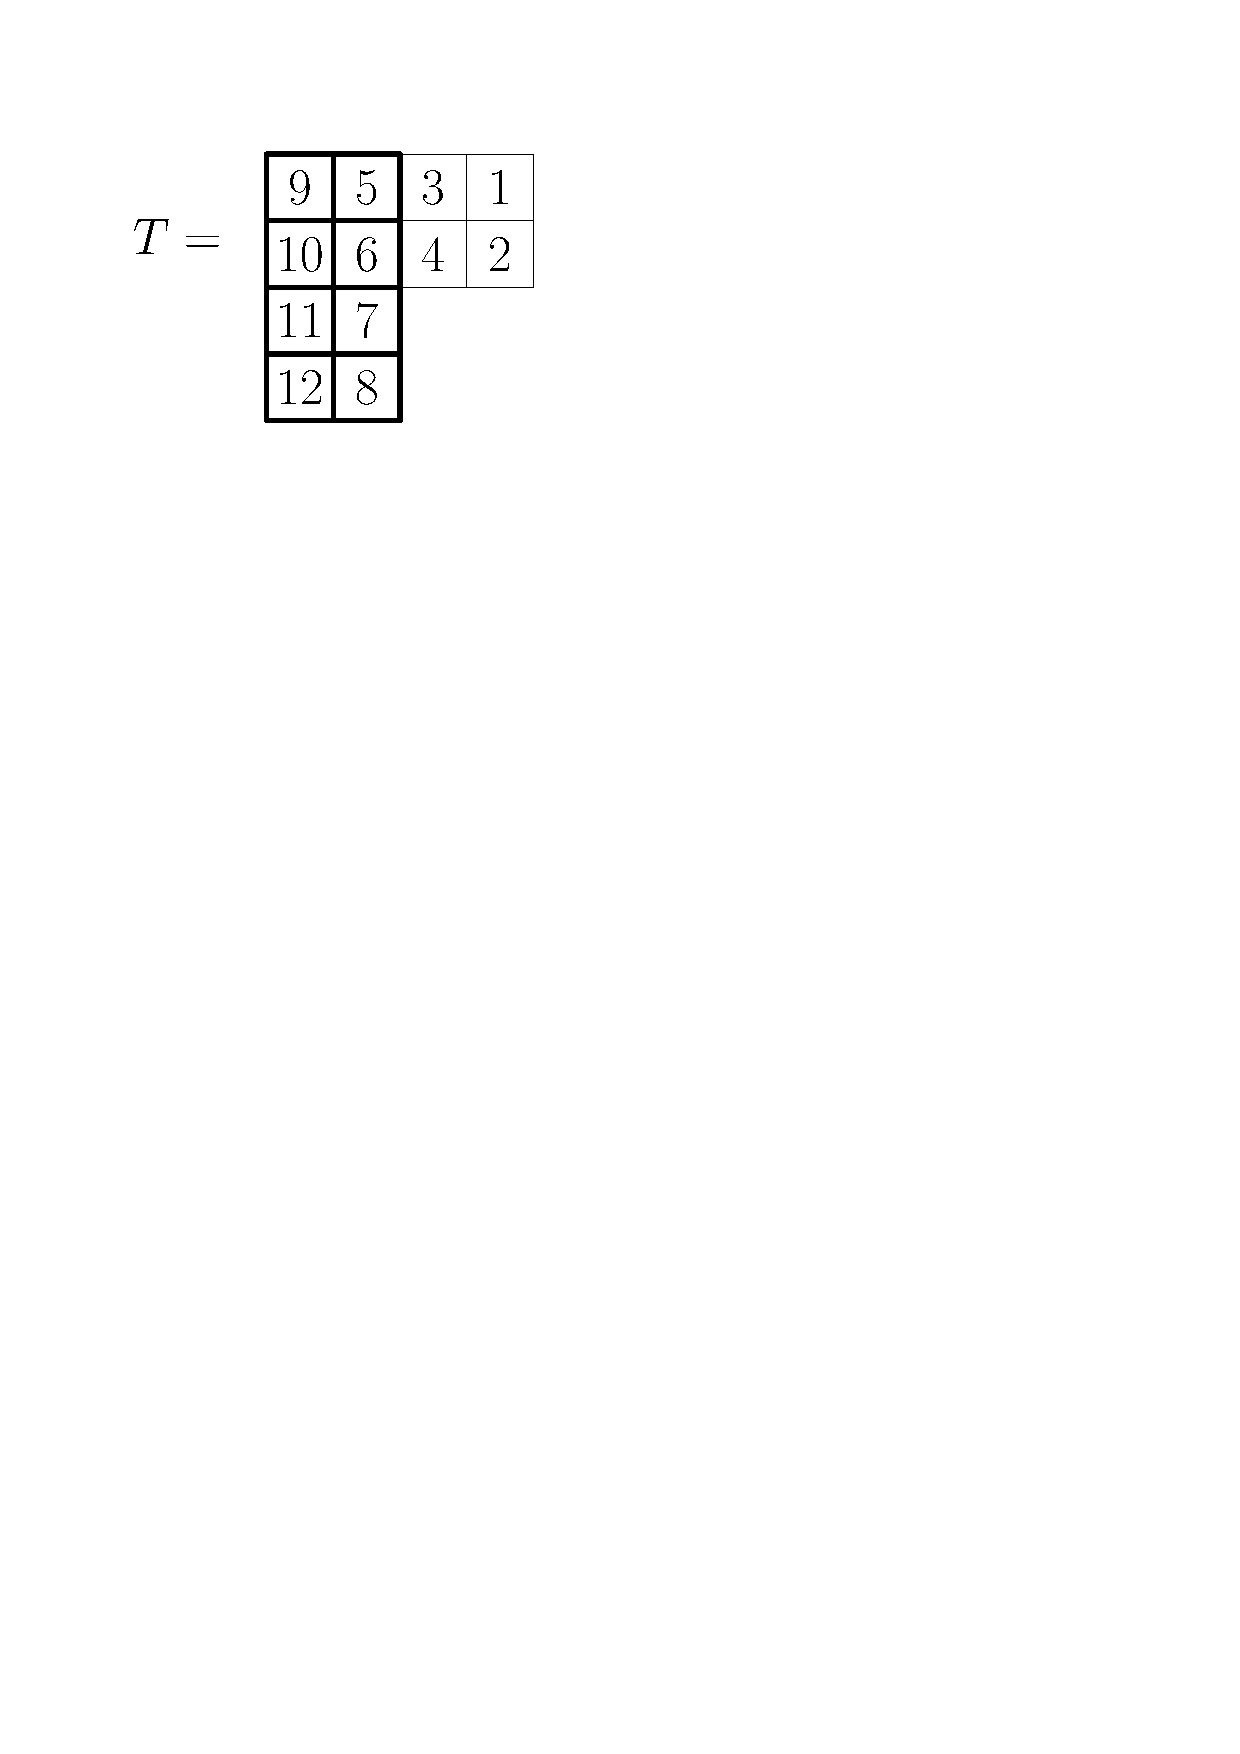
\includegraphics[scale=0.45]{Figures/UFillingExample.pdf}.
\]



If $i=2$ and $v=af_1$, then $U = U_{i,v}$ is given by the matrix (in terms of the basis $f_1,\ldots,f_{12}$):
\setcounter{MaxMatrixCols}{12}
\begin{align}
    U=\begin{bmatrix}
    1 & a & 0 & 0 & 0 & 0 & 0 & 0 & 0 & 0 & 0 & 0 \\
    0 & 1 & 0 & 0 & 0 & 0 & 0 & 0 & 0 & 0 & 0 & 0 \\
    0 & 0 & 1 & a & 0 & 0 & 0 & 0 & 0 & 0 & 0 & 0 \\
    0 & 0 & 0 & 1 & 0 & 0 & 0 & 0 & 0 & 0 & 0 & 0 \\
    0 & 0 & 0 & 0 & 1 & a & 0 & 0 & 0 & 0 & 0 & 0 \\
    0 & 0 & 0 & 0 & 0 & 1 & 0 & 0 & 0 & 0 & 0 & 0 \\
    0 & 0 & 0 & 0 & 0 & 0 & 1 & 0 & 0 & 0 & 0 & 0 \\
    0 & 0 & 0 & 0 & 0 & 0 & 0 & 1 & 0 & 0 & 0 & 0 \\
    0 & 0 & 0 & 0 & 0 & 0 & 0 & 0 & 1 & a & 0 & 0 \\
    0 & 0 & 0 & 0 & 0 & 0 & 0 & 0 & 0 & 1 & 0 & 0 \\
    0 & 0 & 0 & 0 & 0 & 0 & 0 & 0 & 0 & 0 & 1 & 0 \\
    0 & 0 & 0 & 0 & 0 & 0 & 0 & 0 & 0 & 0 & 0 & 1
    \end{bmatrix}.
\end{align}

\end{example}

\begin{example}\label{ex:NTransposeShift}
Let $n = 5$, $\lambda = (2, 1)$, $s = 3$, and let $T$ be as shown in Figure~\ref{fig:NTransposeShift}.
If $i = 4$ and $v = f_8+2f_3+f_1$, then $U = U_{i,v}$ takes $f_j \mapsto f_j$ for all $j \ne 10, 11$, and
\begin{alignat}{3}
    U(f_{10}) &= f_{10} + v &= f_{10} + f_8 + 2f_3 + f_1, \\
    U(f_{11}) &= f_{11} + N_T^t(v) &{}= f_{11} + f_9 + 2f_6 + f_2.
\end{alignat}
We may visualize the basis vectors that appear in $U(f_{10})$ and $U(f_{11})$ with the middle and right diagrams in Figure~\ref{fig:NTransposeShift},
where the indices of the basis vectors that appear in $U(f_{10})$ are highlighted on the left, the basis vectors of $U(f_{11})$ are highlighted on the right, and the indices of the leading terms $f_{10}$ and $f_{11}$ are circled. Note that in general the extra summand in the definition of $U(f_{T(p,q)})$ in the $p=i$ case is ``$v$ shifted left by $\Lambda^i-q$ cells'' and that this definition depends on $T$.
\end{example}

\begin{figure}[t]
    \centering
    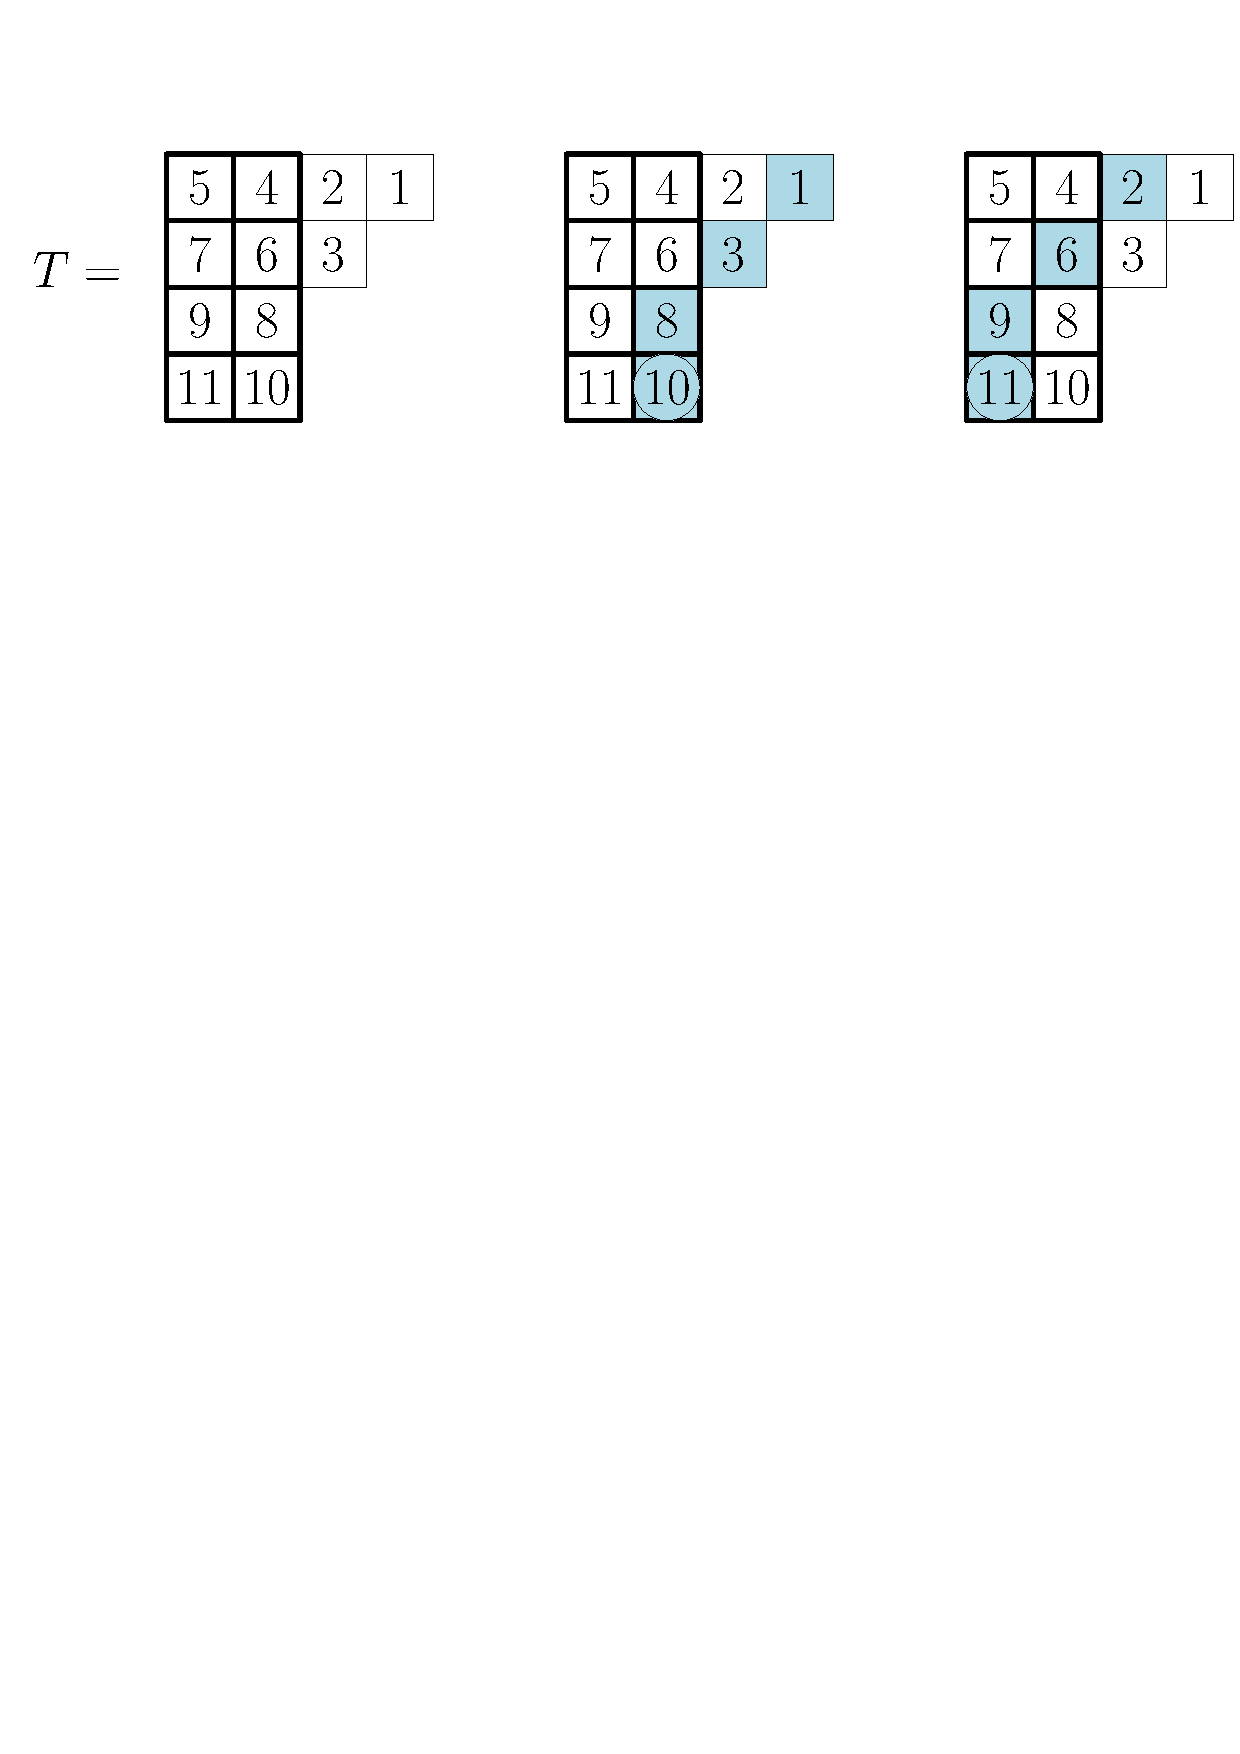
\includegraphics[scale=0.45]{Figures/NTransposeShift.pdf}
    \caption{The Schubert-compatible filling $T$ used in Example~\ref{ex:NTransposeShift} on the left, and illustrations of the basis vectors that appear in $U(f_{10})$ and $U(f_{11})$ in the middle and right, respectively.}
    \label{fig:NTransposeShift}
\end{figure}

\begin{lemma}\label{lem:InvertibleTransf}
Let $U = U_{i,v}$ be the linear map defined in Definition \ref{newdef:InvertibleTransf}. Then $U$
is unipotent, is upper triangular with respect to the ordered basis $f_1,\ldots,f_K$, and satisfies the equation $N_TU = UN_T$.
\end{lemma}

\begin{proof}
It suffices to check the following two properties for each $p$:
\begin{enumerate}
    \item $Uf_p$ is of the form $Uf_p = f_p + \sum_{h< p} a_h f_h$, and
    \item $N_TUf_p = UN_Tf_p$.
\end{enumerate}
First, in the case $p = T(i',j)$ for $i'\neq i$, as in \eqref{neweq:InvertibleTransfEq1}, properties (1) and (2) trivially hold. Second, in the case $p=T(i,\Lambda_i)$, as in \eqref{neweq:InvertibleTransfEq2}, then (1) follows by our choice of $v$ and condition (S5) of Schubert compatibility. Furthermore, (2) holds because both sides are zero.

Finally, suppose $p = T(i,j)$ for $j<\Lambda_i$, as in \eqref{neweq:InvertibleTransfEq3}. Then $(i, j)$ is not the rightmost cell in its row, and we have by definition
\begin{equation}
Uf_{T(i, j)} = N_T^t U f_{T(i, j+1)}.
\end{equation}
By reverse induction on $j$, property (1) holds for $p=T(i,j+1)$. Property (1) for $p=T(i,j)$ then follows by condition (S6) of Schubert compatibility and the fact that $f_{T(i, j)} = N_T^t f_{T(i, j+1)}$.

It remains to show property (2) holds in this case. By the choice of $v$ and reverse induction on $j$, all the terms of the expansion of $Uf_{T(i,j+1)}$ in property (1) correspond to cells of $T$ in column $j+1$ and to the right. In particular,
\begin{equation} \label{eq:column j+1}
U f_{T(i, j+1)} \in \mathrm{im}(N_T).
\end{equation}
We compute
\begin{align}
    (UN_T - N_TU)f_{T(i, j)} &= U(N_Tf_{T(i, j)}) - N_T (U f_{T(i, j)}) \\
    &= U (f_{T(i, j+1)}) - N_T (N_T^t U f_{T(i, j+1)}) \text{ (by \eqref{neweq:InvertibleTransfEq3})}\\
    &= (I - N_TN_T^t) U f_{T(i, j+1)},
\end{align}
which is zero because $I - N_T N_T^t$ vanishes on $\mathrm{im}(N_T)$. Thus, property (2) holds.
\end{proof}

We extend the definition of $\fl_T^{(i)}$ so that it is also a function on admissible injective maps.  In particular, let $w$ be admissible with respect to $T$, and let $w(1) = T(i, \Lambda_i)$. Define 
\begin{align}
    \fl_T^{(i)}(w): [n-1] \rightarrow [K-1] & \text{ if } i\leq \ell(\lambda),\\
    \fl_T^{(i)}(w): [n-1] \rightarrow [K-s] & \text{ if } i>\ell(\lambda)
\end{align}
to be the injective maps where $\fl_T^{(i)}(w)(j)= \fl_T^{(i)}(w(j+1))$ for $1\leq j\leq n-1$.
It is not hard to check directly that if $w$ is admissible with respect to $T$, then $\fl_T^{(i)}(w)$ is admissible with respect to $T^{(i)}$. This also follows from the next lemma.



\begin{definition}
 Define linear maps
\begin{align}
    \phi^{(i)} : \bC^{K-1} \to \bC^K & \,\,\,\text{  for  }i\leq \ell(\la),\\
    \phi^{(i)} : \bC^{K-s} \to \bC^K & \,\,\,\text{  for  }i > \ell(\la),
\end{align}
by setting $\phi^{(i)}(f_j) \coloneqq f_{(\fl_T^{(i)})^{-1}(j)}$ and extending linearly.
\end{definition}

\begin{lemma}\label{lem:CellRecursion}
We have an isomorphism
  \begin{equation}
\Phi: \vspan\{f_{T(h,\Lambda_h)}\st h<i\} \times (C_{\fl_T^{(i)}(w)} \cap Y_{T^{(i)}}) \to C_w\cap Y_T,
 \end{equation}
with the flag $\Phi(v, V_\bullet)$ defined by, for $j=1, \ldots, n$,
\begin{equation}
\Phi(v, V_\bullet)_j := U_{i,v}\big(\vspan\{f_{w(1)}\} + \phi^{(i)}V_{j-1}\big).
\end{equation}
In particular, inverting $\Phi$ gives an isomorphism
 \begin{equation}
 C_w \cap Y_T \cong \bC^{i-1} \times (C_{\fl^{(i)}_T(w)}\cap Y_{T^{(i)}}).
 \end{equation}
\end{lemma}

\begin{proof}
We first show that the image of $\Phi$ is indeed contained in $C_w\cap Y_T$.
First, let $V_\bullet \in C_{\fl_T^{(i)}(w)}\cap Y_{T^{(i)}}$. We examine $\Phi(0, V_\bullet)$. Since $U_{i,0}$ is the identity map, we have for each $j$
\begin{align}
    \Phi(0,V_\bullet)_j =  \vspan\{f_{w(1)}\} + \phi^{(i)}(V_{j-1}).
\end{align}
Since $\fl^{(i)}_{T}$ is order preserving, $\dim(\phi^{(i)}(V_j)\cap F_m)=\dim(V_j\cap F_{\fl^{(i)}_{T}(m)})$ for $m$ in the domain of $\fl_T^{(i)}$, so $\Phi(0,V_\bullet) \in C_w$. Since $w$ is admissible, $F_k \subseteq \Phi(0, V_\bullet)_n$. Next, we check that $\Phi(0, V_\bullet)$ is preserved by $N_T$. For $j=1$, we have $N_Tf_{w(1)} = 0$. For $j \geq 2$, we use the fact that for any $z$ in the domain of $\phi^{(i)}$, $N_T\phi^{(i)}(z)=\alpha f_{w(1)} + \phi^{(i)}N_{T^{(i)}}(z)$ for some $\alpha\in\mathbb{C}$. We calculate:
\begin{align}
    N_T\big(\vspan\{f_{w(1)}\} + \phi^{(i)}V_{j-1}\big) &= N_T \phi^{(i)}V_{j-1} \\
    &\subseteq \vspan\{f_{w(1)}\} +  \phi^{(i)}N_{T^{(i)}}V_{j-1} \\
    &\subseteq \vspan\{f_{w(1)}\} +  \phi^{(i)}V_{j-2}.
\end{align}
Hence, $\Phi(0, V_\bullet) \in C_w \cap Y_T$.

Now let $v\in \vspan\{f_{T(h,\Lambda_h)}\st h<i\}$ be arbitrary. Observe that $\Phi(v,V_\bullet) = U_{i,v}\Phi(0,V_\bullet)$, where $U_{i,v}$ acts on the partial flag $\Phi(0,V_\bullet)$ by acting on each subspace. Since $U_{i,v}$ is upper triangular by Lemma~\ref{lem:InvertibleTransf}, it preserves the Schubert cell $C_w$, so $\Phi(v,V_\bullet)\in C_w$, and (since $w$ is admissible) $F_k \subseteq \Phi(v,V_\bullet)_n$. Finally, since $U_{i,v}$ commutes with $N_T$ by Lemma~\ref{lem:InvertibleTransf}, $N_T$ preserves $\Phi(v, V_\bullet)$:
\begin{equation}
N_T\Phi(v,V_\bullet)_j = N_TU_{i,v}\Phi(0,V_\bullet)_j = U_{i,v}N_T\Phi(0,V_\bullet)_j \subseteq U_{i,v}\Phi(0,V_\bullet)_{j-1} = \Phi(v,V_\bullet)_{j-1}.
\end{equation}
Hence, $\Phi(v, V_\bullet) \in C_w \cap Y_T$.

In order to show that $\Phi$ is an isomorphism, we show that $\Phi$ has an inverse. Define the linear map $\psi^{(i)} \coloneqq (\phi^{(i)})^t$, the transpose with respect to the ordered basis $\{f_j\}$. Explicitly, $\psi^{(i)}$ is the linear map
\begin{align}
    \psi^{(i)} : \bC^K \to \bC^{K-1} & \,\,\,\text{  for  }i\leq \ell(\la),\\
    \psi^{(i)} : \bC^K \to \bC^{K-s} & \,\,\,\text{  for  }i>\ell(\la)
\end{align}
defined by $\psi^{(i)}(f_j) \coloneqq f_{\fl_T^{(i)}(j)}$ if $j$ is in the domain of $\fl_T^{(i)}$ and $0$ otherwise.

Given $V^\prime_\bullet\in C_w\cap Y_T$, note that $\dim(V^\prime_1\cap F_{w(1)})=1$ and $\dim(V^\prime_1\cap F_{(w(1)-1)})=0$, so 
\begin{equation}
    V^\prime_1 = \vspan\{f_{w(1)} + v\} = U_{i,v} \vspan\{f_{w(1)}\}
\end{equation}
for some vector $v = \sum_{h=1}^{i-1} \alpha_h f_{T(h,\Lambda_h)}$, where $\alpha_h\in\mathbb{C}$ are some coefficients. Now note that $f_{w(1)}\in U^{-1}_{i,v}V^\prime_j$ for all $j$ and, in the case $i>\ell(\la)$, we have $V^\prime_j\subseteq \vspan\{f_{T(h,m)}\mid m>1 \mbox{ if } h\neq i\}$.
Hence,
\begin{equation}
U^{-1}_{i,v}V^\prime_j = \vspan\{f_{w(1)}\} + \phi^{(i)}(\psi^{(i)}(V^\prime_j)),
\end{equation}
and from this equality, a routine check shows that the inverse of $\Phi$ is given by
\begin{align}
    \Phi^{-1}(V^\prime_\bullet) = (v, (\psi^{(i)}U^{-1}_{i,v}(V'_2)\subseteq\cdots\subseteq\psi^{(i)}U^{-1}_{i,v}(V'_n))).
\end{align}
Note that the entries of $U_{i,v}$ are regular functions on $Y_T \cap C_w$ (see Section \ref{subsec:Flags}). Moreover, since $U_{i,v}$ is unipotent and upper triangular, the same is true of $U_{i,v}^{-1}$. Thus $\Phi$ and $\Phi^{-1}$ are algebraic maps, so $\Phi$ is an isomorphism of algebraic varieties.
\end{proof}

\begin{remark}[Combined isomorphism $\Phi$]\label{rmk:CombinedIso}
For a fixed $i$, the map $\Phi$ above works the same way for all $w$ such that $w(1) = i$; specifically, the map $U_{i,v}$ depends on $v$ and $i$ but not (the rest of) $w$. As such, all of these $\Phi$'s can be combined into a larger isomorphism. We let
\begin{equation}
    Y_T^i := \big\{V_\bullet \in Y_T : V_1 \subseteq \vspan\{f_{T(h,\Lambda_h)}\st h <i\}\big\} \subseteq Y_T.
\end{equation}
Then we obtain a combined isomorphism
\begin{equation}
    \Phi : \vspan\{f_{T(h,\Lambda_h)}\st h <i\} \times Y_{T^{(i)}} \to Y_T^i \setminus Y_T^{i-1}.
\end{equation}

By induction, $Y_T^i \setminus Y_T^{i-1}$ is a union of cells, as in the definition of affine paving \eqref{eq:affine-paving}. We give the precise characterization of cells in this affine paving below in Theorem \ref{thm:AffinePavingY} and Corollary \ref{cor:AffinePavingFillings}.
We do not use the notation $Y_T^i$ elsewhere in the paper, though we use a restriction of the combined map $\Phi$ in Section~\ref{sec:IrreducibleComponents}. 
\end{remark}

\begin{example}\label{ex:274813cell}
Let $n$, $\lambda$, $s$, and $T$ be as in Example~\ref{ex:6223unip}.  Let $w=2\, 7 \, 4\, 8\, 1\, 3$, which is admissible with respect to $T$. Then $i=w(1) = 2$. A flag $V_\bullet\in C_w\cap Y_T$ can be represented by a matrix
\begin{align} \label{eq:CoordinateExampleEq}
    \begin{bmatrix}
    a & c & d & g & 1 & 0 \\
    1 & 0 & 0 & 0 & 0 & 0 \\
    0 & ab& a & de & 0 & 1 \\
    0 & b & 1 & 0 & 0 & 0 \\
    0 & 0 & 0 & ae & 0 & 0 \\
    0 & 0 & 0 & e & 0 & 0 \\
    0 & 1 & 0 & 0 & 0 & 0 \\
    0 & 0 & 0 & 1 & 0 & 0 \\
    0 & 0 & 0 & 0 & 0 & 0 \\
    0 & 0 & 0 & 0 & 0 & 0 \\
    0 & 0 & 0 & 0 & 0 & 0 \\
    0 & 0 & 0 & 0 & 0 & 0
    \end{bmatrix},
\end{align}
where each $V_j$ is the span of the first $j$ columns, and $a$, $b$, $c$, $d$, $e$, and $g$ are arbitrary elements of $\mathbb{C}$. Identifying $\vspan\{f_{1}\}\cong \bC^1$, the map $\Phi^{-1}$ sends this matrix to the pair $(af_1,V_\bullet')$, where the flag $V'_\bullet$ is represented by
\begin{align}
    \begin{bmatrix}
    c & d & g & 1 & 0 \\
    0 & 0 & de & 0 & 1 \\
    b & 1 & 0 & 0 & 0 \\
    0 & 0 & 0 & 0 & 0 \\
    0 & 0 & e & 0 & 0 \\
    1 & 0 & 0 & 0 & 0 \\
    0 & 0 & 1 & 0 & 0 \\
    0 & 0 & 0 & 0 & 0 \\
    0 & 0 & 0 & 0 & 0 \\
    0 & 0 & 0 & 0 & 0 \\
    0 & 0 & 0 & 0 & 0
    \end{bmatrix}.
\end{align}
\end{example}



\begin{theorem}\label{thm:AffinePavingY}
If $T$ is Schubert compatible, then the intersections $C_w\cap Y_{n,\la,s,T}$ for $w$ admissible are the cells of an affine paving of $Y_{n,\la,s,T}$.
\end{theorem}

\begin{proof}
Since the Schubert cells $C_w$ are the cells of an affine paving of $\Fl_{(1^n)}(\bC^K)$, it suffices to show that each nonempty intersection $C_w\cap Y_{n,\la,s,T}$ is isomorphic to an affine space $\bC^d$ for some $d$. By Lemma~\ref{lem:CellRecursion}, $C_w\cap Y_{n,\la,s,T}$ is nonempty if and only if $w$ is admissible. We proceed by induction on $n$ to show that each of these intersections is an affine space.



In the base case when $n=0$, we have $n = k = 0$, $\lambda = \Lambda = \emptyset$ and $s > 0$ is arbitrary. Then $\bC^K = \bC^0$ and $Y_{n, \lambda, s, T} = \Fl_\emptyset(0) = \{\mathrm{pt}\}$. Thus, the only nonempty intersection is a single point.

In the inductive case where $n\geq 1$, we have
\begin{equation}
    C_w\cap Y_{T}\cong \mathbb{C}^{i-1}\times (C_{\fl_T^{(i)}(w)}\cap Y_{T^{(i)}})
\end{equation}
by Lemma~\ref{lem:CellRecursion}.  By induction, 
$C_{\fl_T^{(i)}(w)}\cap Y_{T^{(i)}}\cong \mathbb{C}^m$ for some $m$, so $C_w\cap Y_T \cong \bC^{i+m-1}$, and our induction is complete.
\end{proof}



\begin{definition}
An \textbf{injective partial row-decreasing filling} of $[\Lambda]$ is a filling of a subset of the cells of $[\Lambda]$ with the labels $1,2,\dots, n$ (without repeating any labels) such that the filled cells are right justified in their row, the labeling decreases along each row, and each cell of $[\lambda]$ is filled.

Given $w$ admissible with respect to $T$, let $\operatorname{IPRD}_T(w)$ be the injective partial row-decreasing filling of $[\Lambda]$ such that, for $1\leq i\leq n$, if $w(i) = T(a,b)$, then the cell $(a,b)$ of $[\Lambda]$ is labeled with $w(i)$.
\end{definition}

\begin{figure}[t]
  \centering
  \includegraphics[scale=0.45]{Figures/RowDecreasingBijection.pdf}
  \caption{With $T$ in reading order as shown on the left, an example of the bijective correspondence between admissible functions and injective partial row-decreasing fillings on the right.\label{fig:FillingBijectionExample}}
\end{figure}

Note that the data of an admissible $w$ with respect to $T$ is equivalent to the data of the corresponding IPRD.  See Figure~\ref{fig:FillingBijectionExample} for an example of this correspondence. Combining this with Theorem~\ref{thm:AffinePavingY}, we have the following corollary.

\begin{corollary}\label{cor:AffinePavingFillings}
The nonempty cells in the affine paving of Theorem~\ref{thm:AffinePavingY} are in bijection with injective partial row-decreasing fillings of $[\Lambda]$.
\end{corollary}




\section{Pavings of projected $\Delta$-Springer varieties}

\SG{To do: show that the same paving idea gives a paving of the projected versions of a $\Delta$-Springer variety, and the paving works over $\bk$.}

Let $\bk$ be a field.

\begin{definition}
Let $N_\Lambda$ be a nilpotent matrix with entries in $\bk$ of Jordan type $\Lambda$. Given $\beta$ a (strong) composition of $n$, define the \textbf{projected $\Delta$-Springer variety}
\begin{align}
    Y_{n,\la,s}^\beta(\bk)\coloneqq \{V_\bullet \in \Fl^{\beta}(\bk^K)\st N_\Lambda V_i\subseteq V_{i}\text{ for }i\leq \ell(\beta),\text{ and }N_\Lambda^{n-k}\bk^K\subseteq V_n\},
\end{align}
where $V_0\coloneqq 0$.
\end{definition}

\begin{theorem}
There is an affine paving of $Y_{n,\la,s}^\beta(\bk)$, with cells given by the nonempty intersections $C_w \cap Y_{n,\la,s}^\beta(\bk)$, as $w$ runs over all injective functions $[n]\to [K]$ that are increasing on the parts of $\beta$.
\end{theorem}

\begin{theorem}
The nonempty intersections from the previous theorem are characterized by those $w$ that are both admissible with respect to $T$ and are increasing on the parts of $\beta$.
\end{theorem}

\begin{definition}
Given $w$ an injective function $[n]\to [K]$ admissible with respect to $T$, let $\inv_T(w)$ be the number of pairs\dots in $\IPRD(w)$.\SG{finish this}
\end{definition}

\begin{theorem}
For $w$ admissible with respect to $T$ and $\beta$, 
\[
\dim_\bk(C_w\cap Y_{n,\la,s}^\beta(\bk)) = \inv_T(w).
\]
\end{theorem}

\begin{theorem}
We have
\[\Frob(R_{n,\la,s};q) = \sum_{\beta}|Y_{n,\la,s}^\beta(\Fq)|\, m_\beta(\bx).\]
\end{theorem}

\section{Decomposing the $\Delta$-Springer variety into \\Springer fibers crossed with affine spaces}

\begin{definition}
Let $T$ be the filling of $[\Lambda]$ given by right-justified reading order. Given $\alpha$ a (strong) composition of $n$ into $s$ parts that contains $\la$, let $\bk^\alpha\subseteq \bk^K$ be the subspace spanned by $f_{i}$ for $i$ a label of $T$ contained in $[\alpha]$. Define
\begin{align*}
    \cB^\beta_\alpha(\bk) \coloneqq \{V_\bullet \in Y_{n,\la,s}^\beta(\bk) \st V_n = \bk^\alpha\}.
\end{align*}
\end{definition}
Note that it follows from the definition that $\cB_\alpha^\beta(\bk)$ is isomorphic to a Springer fiber, $\cB_\alpha^\beta(\bk)\cong \cB_{\sort(\alpha)}(\bk)$.

Let $C_w^{(n)}$ be the Schubert cell in the Grassmannian $\Fl^{(n)}(\bk^K)$.

\begin{theorem}
We have
\[
\{V_\bullet\in Y_{n,\la,s}^\beta(\bk)\st V_n\in C_w^{(n)}\}\cong \bk^m\times \cB_\alpha^{\beta}(\bk),
\]
where $m = \sum_i(s-\alpha_i')(\alpha_{i+1}'-\la_{i+1}') + \coinv(\alpha)$.
\end{theorem}

\end{document}